\documentclass[a4paper,10.0pt,twoside]{npr}

\usepackage{multicol,graphicx,lastpage,footmisc,fancyhdr,paralist,
tabularx,array,booktabs,caption,multirow,upgreek,mathrsfs,gensymb,color}
\usepackage[fancyhdr,space,fntef,fontset=ubuntu]{ctex}
\usepackage{amssymb,bm,mathrsfs,bbm,amscd}
\usepackage{flushend,cuted}
\usepackage{refcount}
\usepackage{savesym}
\usepackage{textcomp}
\usepackage[tbtags]{amsmath}  %
\savesymbol{iint}
\usepackage{amstext} %数学宏包文本命令
\usepackage{balance} %版心底部对齐

\flushbottom      %版心底部对齐
\setcounter{section}{0}
\begin{document}
%\begin{CJK*}{GBK}{\song}{\wuhao}{\rm}

%___________________________________________________________________________________
\def\rd{{\rm d}}

\newcommand{\RM}{\ensuremath{\mathrm}}   %正体 既可用于文本模式也可用于数学模式
\newcommand{\dif}{\mathrm{d}}  %直立体d
\newcommand{\me}{\mathrm{e}}  %直立体e
\newcommand{\mi}{\mathrm{i}}  %直立体i
\newcommand{\mj}{\mathrm{j}}  %直立体j
\newcommand{\afrac}[2]{\dfrac{\,#1\,}{\,#2\,}}  %略长分数线
\newcommand{\nn}{\nonumber}  %公式无编号
\newcommand{\nt}{\noindent}
\newcommand{\OO}{~\text{。}}
\newcommand{\PP}{~\text{,}}
\newcommand{\OP}{~\text{;}}
\newcommand{\LT}{\left}
\newcommand{\RT}{\right}

%___________________________________________________________________________________

\balance
\fancypagestyle{myfoot}
{%
\fancyhf{}
\fancyhead[c]{\wuhao\song 高~等~核~物~理~实~验}
\renewcommand{\headrule}{\vskip 2pt
\hrule height0.4pt width\headwidth \vskip1pt
\hrule height0.4pt width\headwidth \vskip-1.8pt}
}%
\thispagestyle{myfoot}

%%%%%%%%%%%%%%%%%%%%%%%%%%%%%%%%%%%%%%%%%%%%%%%%%%%%%
%    奇偶页眉
%%%%%%%%%%%%%%%%%%%%%%%%%%%%%%%%%%%%%%%%%%%%%%%%%%%%%
\pagestyle{fancy}
\fancyhead{}
\fancyhead[ce]{\xiaowu\song \hspace{0.5em}高~等~核~物~理~实~验}
%\fancyhead[ro,le]{\xiaowuhao \hspace{0.5em}\textbf{\textperiodcentered}\;\thepage\;\textbf{\textperiodcentered}\hspace{0.5em}}
%\fancyhead[ce]{\xiaowu\song 粒~子~物~理~与~原~子~核~物~理~专~题~实~验}
%\fancyhead[re]{\xiaowu\song \hspace{0.5em}第\;31\;卷\hspace{0.5em}}
\fancyfoot[ce,co]{}
\renewcommand{\headrule}{\vskip 2pt
\hrule height0.4pt width\headwidth}


\setcounter{page}{001}%
\fancyhead[co]{\xiaowuhao\song  乔颢:位置灵敏塑料闪烁体谱仪}    %奇页页眉
\begin{center}
\title{%
\xiaoerhao \bf  %章标题为两行时改为 \exiaoer
$^{90}_{38}Sr$位置灵敏塑料闪烁体谱仪\\[-5mm]}
\maketitle
\large \fs
乔颢$^{^1}$\\[2mm]

\xiaowu \song
1. 北京大学物理学院,海淀区 北京 100871;\\[4mm]

 
\footnotetext[0]{{\bf 作者简介:}~~\begin{minipage}[t][4.2mm]{149mm}\song
乔颢,E-mail: i@catofes.com
\end{minipage} }
%\footnotetext[0]{{\bf 通信作者:}\song ~~E-mail: xxx@xxx.xxx }%通信作者为第一作者时不要此项

\parbox{158mm} {
\zywu{\bf 摘要:}~~\fs
该实验使用塑料闪烁体,利用PMT读出不同位置收到信号的时间,通过后续电子学处理成功重建了事件的位置信息。标定得到事件发生位置与多道读出峰位的关系为$l=-0.433x+287.8(cm)$,并且计算得到信号在闪烁体内传播的速度为$1.48\times10^{8}m/s$。 重建待测事件位置分别为20.5cm以及64.8cm,与真实值22cm和65cm较为接近。

{\bf 关键词:}~~\fs 位置重建,塑料闪烁体,分辨}\\
\end{center}
%%%%6.正文
\vspace{5mm}
%%%%6.正文
\setcounter{section}{0}
\begin{multicols}{2}
%----------------
%____________________________________________________________________________
%%%%以上请不要改动%%%%%%%%%%%%%%%%%%%%%%%%%%%%%%%%%%%%%%%%%%%%

\section{引言}    %1
\vspace*{-1mm}
\song\wuhao
塑料闪烁体是一种比较理想的信号传导媒介物质。当粒子进入闪烁体后,闪烁体受激发生大量的光子,并在塑料闪烁体内传播。通过合理的设计塑料闪烁体的形状,光导的方式,以及反射体的位置,可以将光信号引入到光电倍增管中从而转换为电子信号而被接受处理。这样通过多个光电倍增管接受闪烁信号,并利用其相对的位置关系,以及对于同一个信号测量得到的时间关系,最终确定事件发生的位置。

在本实验中使用长矩形塑料闪烁体并在其两端安装光电倍增管,可以利用光电倍增管得到信号时间差来确定信号发生的位置。
\section{实验}
\subsection{实验介绍及原理}

利用塑料闪烁体探测器进行位置刻度的方式一般有两种。利用光在闪烁体内传输近似以指数衰减,通过测量信号幅度的大小来重建位置,以及利用光在闪烁体里传输需要一定的时间来进行刻度。对于一个长塑料闪烁体而言,如下图所示:

\begin{center}
   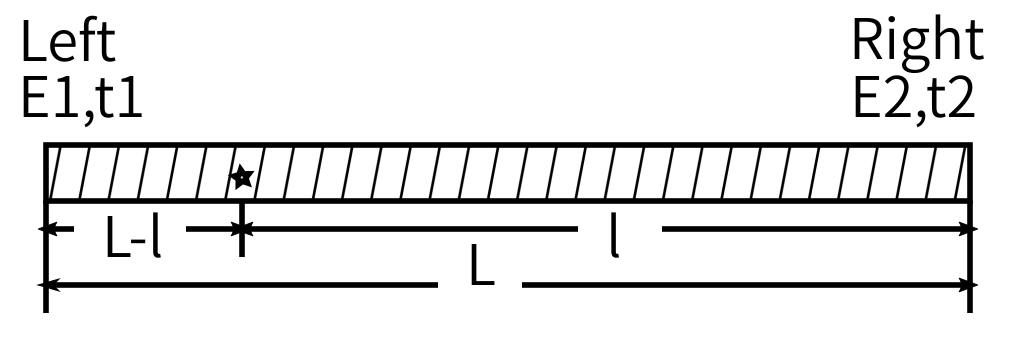
\includegraphics[width=0.45\textwidth]{xinhao.png}
\\
\xiaowu\song 图~1\begin{minipage}[t]{75mm} \quad 塑料闪烁体利用时间信号进行位置刻度原理示意图。\\[-1mm]\wuhao
\end{minipage}
\end{center}
塑料体总长为L,两端接收到信号的时间分别为$t_1$和$t_2$,于是时间差可以表示为
\begin{equation}
	t_\Delta = t_1-t_2 = \frac{L-2l}{v}
\end{equation}
其中$v$是闪烁体中光传播速度。因而可以得到关系
\begin{equation}
	l=\frac{L-vt_\Delta}{2}=offset -\frac{v}{2}t_\Delta
\end{equation}
可见信号距一端的距离与收到信号的时间差成正比关系,而闪烁体的长度则体现在正比关系的截距。所以可以通过时间信息对事件发生的位置进行重建。通过测量已知位置的信号所产生的时间差,可以对探测器进行标定,进而能够通过测量待测事件信号的时间差确定待测事件发生的位置。


\subsection{实验过程}

本实验使用的塑料闪烁体是有高能科迪生产,长为1m左右,衰减时间为2.1ns。粒子激发闪烁产生的光信号经由两端的光电倍增管(PMT)探测输出。具体实验的装置图如下所示:

\begin{center}
   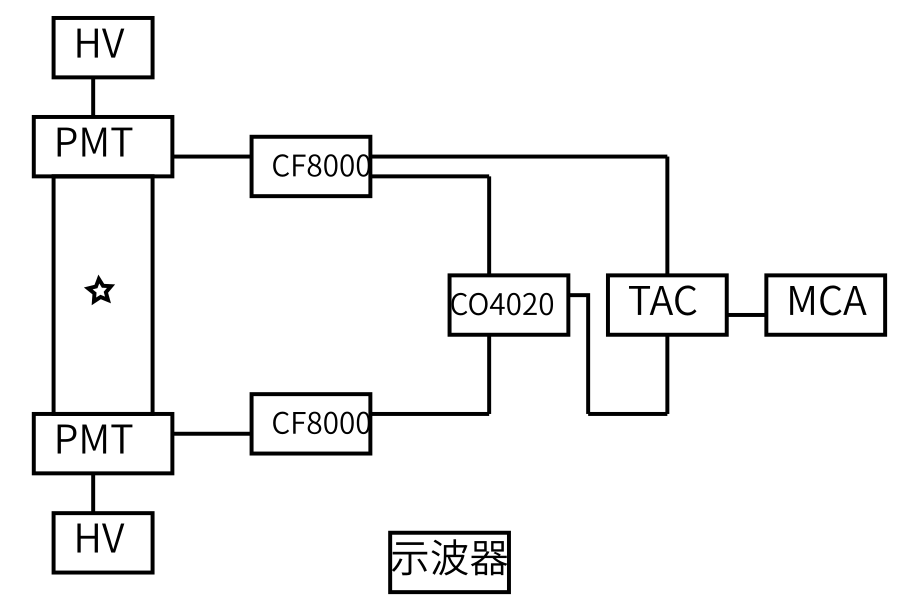
\includegraphics[width=0.45\textwidth]{xianlu.png}
\\
\xiaowu\song 图~2\begin{minipage}[t]{75mm} \quad 塑料闪烁体利用时间信号进行位置刻度连接示意图。\\[-1mm]\wuhao
\end{minipage}
\end{center}

PMT将接收到的光信号转化为电信号并输出,通过恒比定时甄别器(CF8000)转换为数字脉冲信号,并由逻辑符合单元(CO4040)进行逻辑与操作。我们假设从左侧PMT采集并由甄别器输出的是A信号,右侧为B信号,AB信号在符合单元进行符合运算。这样只要在B信号上加上一定的延时,就可以使得符合输出信号的时间为AB信号同时发生的时间。而因为延时导致的信号后移只会影响2式中的offset,对于斜率没有影响。

将符合输出的信号与A路直接输出的信号之间的时间差转换为电压信号,就可以通过多道得到信号时间差,从而能够根据2式标定并重建事件位置了。具体的实验步骤如下:

\begin{enumerate}
\item 根据上图连接实验装置,并利用示波器探测检验各个器件输出的信号,记录相关信息。
\item 不放置放射源测量本底谱,并通过调节PMT的电压使得本底信号对称。
\item 将$^{60}$Co放射源放置在闪烁体上不同的位置,测量时间信号,对探测器进行标定。
\item 将源放置在未知位置,测量并计算出实际位置。
\end{enumerate}

\section{实验结果和讨论}

 首先将PMT电压调整到2.09kV左右,直接利用示波器观察输出信号的波形状况,各个信号之间的特征如下表以及下图所示:



\begin{center}
\bgliu
{\bf 表~1\quad
实验中各个仪器输出信号特点}\\[0.5mm]
\renewcommand{\arraystretch}{1.5}
\liuhao\song\rm
\newcolumntype{M}{>{\centering\arraybackslash}m{12mm} >{\centering\arraybackslash}m{10mm}
>{\centering\arraybackslash}m{10mm}>{\centering\arraybackslash}m{6mm}>{\centering\arraybackslash}m{10mm}>{\centering\arraybackslash}m{12mm}}
\begin{tabular}{M}
\specialrule{0.1em}{1pt}{1pt}

信号来源  &  上升时间/ns &  下降时间/ns  &  幅度 &  宽度/ns  &  时序 \\
\midrule
左PMT&5.2&24&544mV&-&-\\
右PMT&6.4&38&632mV&-&-\\
甄别器&-&-&1.02V&110&左端信号先于右端信号\\
符合&-&-&1.10V&86&左端信号先于右端信号\\
TAC&-&-&3.92V左右&-&-\\
\specialrule{0.1em}{3pt}{2pt}\\[-4mm]
\end{tabular}\\
\renewcommand{\arraystretch}{1.0}
\end{center}

\begin{center}
   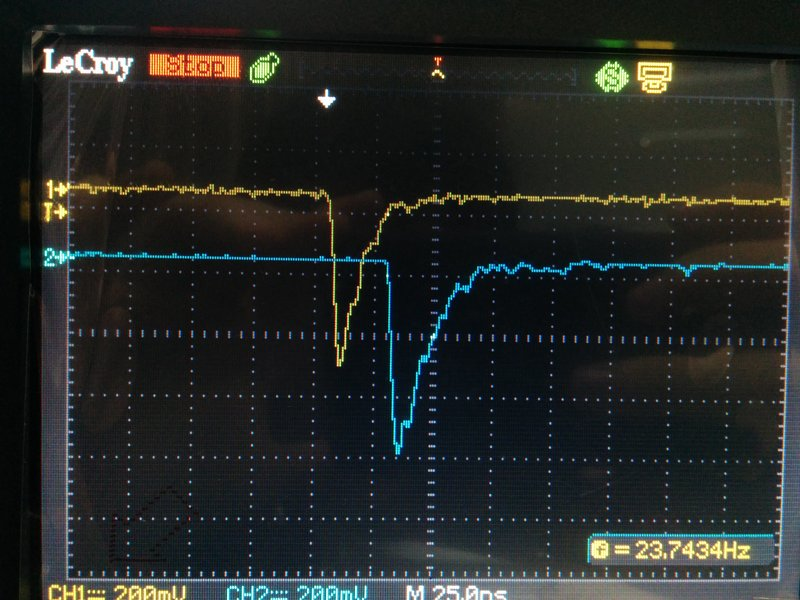
\includegraphics[width=0.4\textwidth]{1.jpg}
\\
\xiaowu\song 图~3\begin{minipage}[t]{75mm} \quad 光电倍增管输出信号。黄线为左端信号,蓝线为右端信号。从PMT输出的是探测到的强度信号,从图中可以看出光闪烁体被激发后迅速发光产生一个信号,并在大约40ns左右信号衰弱消失。\\[-1mm]\wuhao
\end{minipage}
\end{center}
\begin{center}
   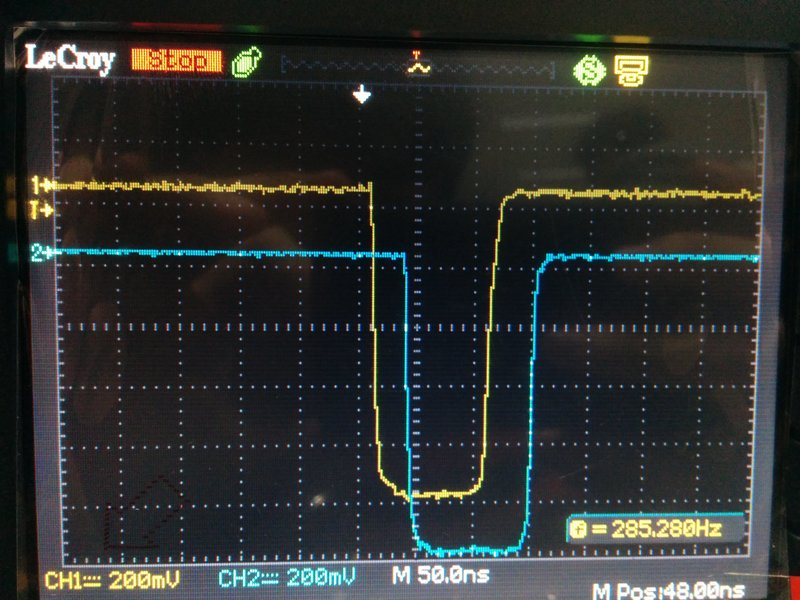
\includegraphics[width=0.4\textwidth]{2.jpg}
\\
\xiaowu\song 图~4\begin{minipage}[t]{75mm} \quad 甄别器输出信号。黄线为左端信号,蓝线为右端信号。PMT输出信号经过甄别器被转换为脉冲信号,此时探测器探测到的能量相关信息被丢弃,只保留时间相关信息。\\[-1mm]\wuhao
\end{minipage}
\end{center}
\begin{center}
   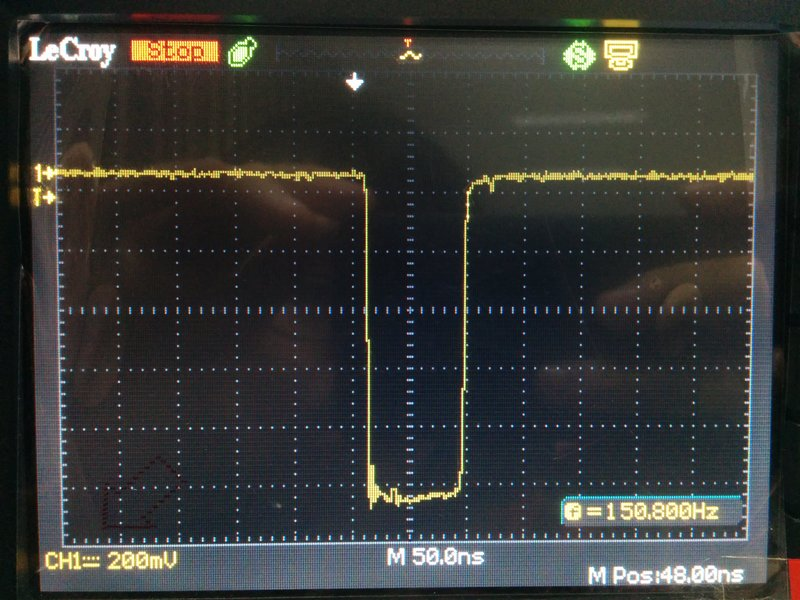
\includegraphics[width=0.4\textwidth]{3.jpg}
\\
\xiaowu\song 图~5\begin{minipage}[t]{75mm} \quad 符合输出信号。可以看出经过符合后,输出信号宽度是小于甄别器给出的信号的。此信号的上升延就表示右端信号发生时刻。\\[-1mm]\wuhao
\end{minipage}
\end{center}
\begin{center}
   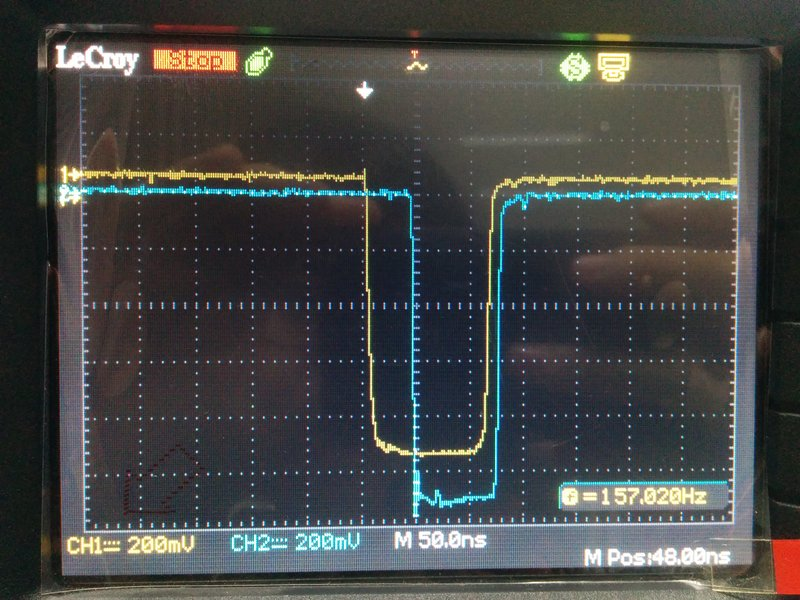
\includegraphics[width=0.4\textwidth]{4.jpg}
\\
\xiaowu\song 图~6\begin{minipage}[t]{75mm} \quad TAC输入信号。黄线为左端信号,蓝线为符合输出信号。两线上升延之间的时间差就是本次测量的时间差$t_\Delta$\\[-1mm]\wuhao
\end{minipage}
\end{center}
\begin{center}
   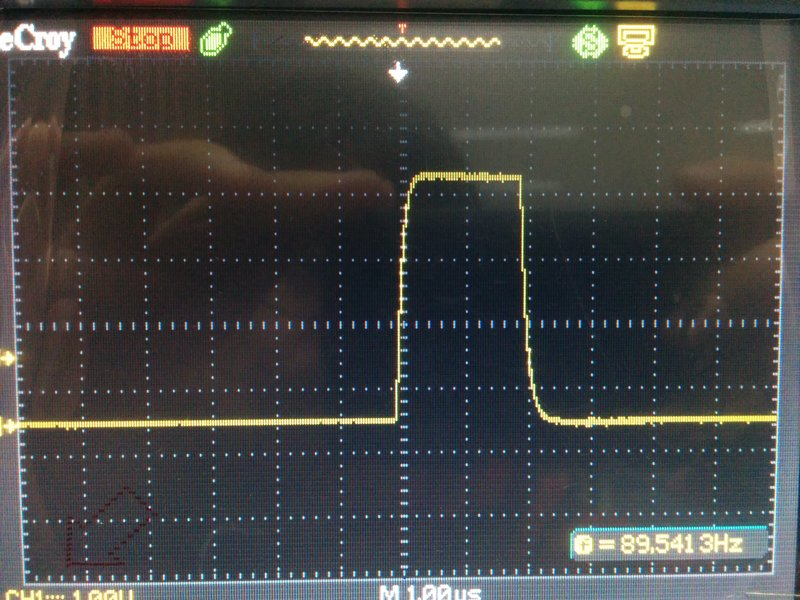
\includegraphics[width=0.4\textwidth]{5.jpg}
\\
\xiaowu\song 图~7\begin{minipage}[t]{75mm} \quad TAC输出信号。TAC负责将时间信息转化为电压信息,这样就可以用多道对时间信息进行后续的处理。\\[-1mm]\wuhao
\end{minipage}
\end{center}

观察完仪器输出后,可以直接测量宇宙射线。因为宇宙射线本身是一个比较均匀的入射事件,因而理论上多道观测到的时间差谱应该会是一个比较均匀的平台。然而实际情况下两个PMT的性能参数并不一致,对事件的敏感程度也不一,从而使测量的平台并不平。因此需要通过调整PMT高压来使得平台平整。调整后的电压信息为:左侧2.09kV,右侧2.06kV。

调整完高压后就可以对探测器进行标定了。将源放在不同的位置,测量得到的结果如下:

\begin{center}
\bgliu
{\bf 表~2\quad
不同位置测量数据,多道为1024道,时间分辨以及位置分辨的计算见后文。10-90cm处的数据是标定数据,22,65cm处的数据是待测数据。}\\[0.5mm]
\renewcommand{\arraystretch}{1.5}
\liuhao\song\rm
\newcolumntype{M}{>{\centering\arraybackslash}m{12mm} >{\centering\arraybackslash}m{12mm}
>{\centering\arraybackslash}m{12mm}>{\centering\arraybackslash}m{12mm}>{\centering\arraybackslash}m{12mm}}
\begin{tabular}{M}
\specialrule{0.1em}{1pt}{1pt}

位置/cm	&	峰道址	&	半高宽	&	时间分辨/ns	&	位置分辨	/cm\\
\midrule
10	&	644	&	35.4	&	2.07	&	15.3	\\
30	&	593	&	36.3	&	2.13	&	15.8	\\
50	&	549	&	35.2	&	2.06	&	15.2	\\
70	&	505	&	40.3	&	2.36	&	17.5	\\
90	&	457	&	38.6	&	2.26	&	16.7	\\
22	&	617	&	38.0	&	2.23	&	16.5	\\
65	&	515	&	37.6	&	2.20	&	16.3	\\
\specialrule{0.1em}{3pt}{2pt}\\[-4mm]
\end{tabular}\\
\renewcommand{\arraystretch}{1.0}
\end{center}

本实验中TAC量程为100ns, 输出10V的电压。多道为1024道,最高接收到6V的电压。所以每道对应的时间为
\begin{equation}
	\delta t=\frac{6/10\times100 ns}{1024}=58ps
\end{equation}
由此可以通过半高宽计算出时间分辨,即为半高宽乘以58ps。
\begin{center}
   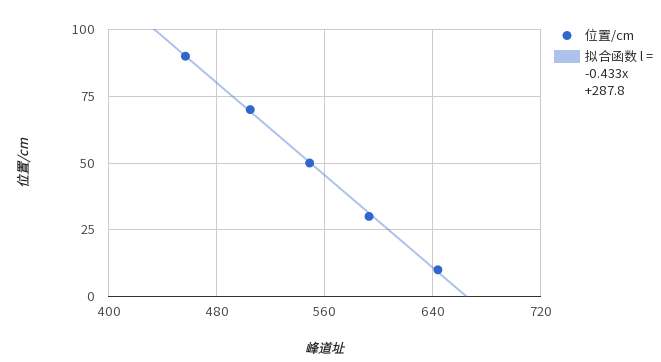
\includegraphics[width=0.45\textwidth]{nihe.png}
\\
\xiaowu\song 图~8\begin{minipage}[t]{75mm} \quad 标定数据位置和峰道址关系图。\\[-1mm]\wuhao
\end{minipage}
\end{center}
通过标定数据的位置以及对应的峰位我们可以计算得到位置与道数的关系。如上图所示,拟合可以得到:
\begin{equation}
	l = -0.433x+287.8 (cm)
\end{equation}
其中x为道址,l为源的位置。由此公式我们可以计算得到不同位置的位置分辨,即利用半高宽乘以0.433即可,同时我们也可以计算出待测事件的位置。计算得到22cm以及65cm附近事件的位置为20.5cm和64.8cm。可以看出两个结果相比较而言,20.5cm的误差更大一些,这个可能是由于该事件更靠探测器边缘,两端PMT接受到的信号差别较大从而使得统计误差较大,因而结果偏离的更远一些。

通过位置和峰位的斜率关系我们可以计算得到光在闪烁体内传播的速度信息。
\begin{equation}
	c'=-k\times\frac{1024\times2}{0.6\times100}=14.8cm/ns
\end{equation}


\section{总结和结论}
本实验中利用塑料闪烁体测量了辐射入射点在闪烁体内的位置。通过在不同的位置放源标定得到源所在的位置与测量结果有以下关系:$l=-0.433x+287.8$。其中x为多道测量得到的峰道址。对于两个未知位置测量的结果分别为20.5cm以及64.8cm。并计算的道光在闪烁体内传播的速度为$1.48\times10^{8}m/s$。
\section{致谢}
感谢楼建玲老师的细致地讲解以及为实验做出的准备。
\section{参考文献}

\noindent
[1] 讲义
\end{multicols}

\newpage


\section*{附录:思考题}
1、$^{60}$Co发生一个$\beta$衰变和两个$\gamma$衰变,塑料闪烁体主要响应的是中子以及$\beta$粒子,对$\gamma$粒子响应不强,因而我觉得用塑料闪烁体测量Co的能谱只能得到其$\beta$谱,而且分辨率可能不会很好。

2、因为塑闪受激发光发出的光是向空间各个方向发光的,恒比定时甄别器甄别出来的不是一个脉冲信号最开始的时候,而是达到一定强度的时候,因而此时光并不之直线传播到达PMT的。光的传播距离加长,时间变长,而我们假设中光的传播距离较短,因而速度测量值较小。

3、低道址的地方地,意味着时间差小的信号弱,因而需要加强这一信号,右端信号晚于左端信号,因而时间差小的时候远靠右侧,此时需要加强符合信号则需要加强左侧PMT探测效率,也就是提高左侧PMT的电压,同理减少右侧PMT电压也可以。

计算时间分辨率可以根据本地平台两侧展宽来估测。假设本底粒子打在塑闪上产生的是一个高斯分布,那么整个能谱图则是多个高斯分布的叠加。在边缘位置的半高宽可以认为就是闪烁体的时间分辨。从数据中读得道数差约为75道(4096道的多道),因而对应的时间分辨率约为2*75/4096*0.6*100=2.2ns。 

较为精确的计算应该是将高斯分布进行积分求出平台应该满足的分布,然后拟合得到高斯分布的$\sigma$。但是本地测量中误使用了4096道多道,无法转成数据文件并处理,因而无法给出更为精确的结果。

4、TAC输出的是正信号,其他的都是负信号。甄别器,符合,TAC输出的是数字方波信号。光电倍增管,甄别器,符合输出的是ns级别信号。

5、测试高频信号中用50欧姆,其他一般用1M欧姆。

6、使用分辨率更好一些的塑闪,使用灵敏度高一些的PMT等。

\clearpage
%\end{CJK*}
\end{document}



